\section{Hypothesis Graph}%
\label{sec:hgraph}
The \ac{hgraph} is responsible for generating action sequences, called hypothesis (consisting of a list of succesive edges from start to target node in the \ac{hgraph}) that complete a single subtasks. When all subtasks in a task are completed, the \ac{hgraph} halts and concludes the task succesfully completed. A search in the joint configuration space is avoided because an edge only operates in a single mode of dynamics, such as driving or pushing. When a object cannot directly be steered toward it's target location new nodes are generated which need to be completed before the original object can be steered toward it's target location. An example of when an object cannot directly be steered toward it's target state is because the path is blocked by another object. An hypothesis, consisting of a list of edges that represent actions in the robot environment might succeed or fail. \Cref{tikz:flowchart_hgraph} displays a flowchart explaining how new nodes and edges are generated in the \ac{hgraph}. Succesfully completed edges eventually result in completed subtasks, failed edges trigger replanning that will restart the search to a hypothesis.\bs

\Cref{subsec:hgraph_definition} defines the \ac{hgraph} and components, then~\cref{subsec:two_loops} eleborates how the \ac{hgraph} searches for a solution in the joint configuration space. Followed by subsections elaborating the methods used by the \ac{hgraph} such as system identification and control methods in \cref{subsec:sys_iden_and_control_methods}, path estimation in \cref{subsec:estimating_path_existence}, motion planning in \cref{subsec:motion_planning}, manipulation planning in \cref{subsec:manipulation_planning} and fault detection in \cref{subsec:fault_detection}.\bs

% For every subtask in a task, a start and a target node is created, the hypothesis graph tries to connect the starting node to the corresponding target node by adding node and edges. The choice and content of these nodes and edges is based on local planning and randomisation, elaborated in~\cref{subsec:estimating_path_existence,subsec:motion_planning,subsec:manipulation_planning}. A successive path from a starting node to the corresponding target node is called a hypothesis. During the search for a hypothesis, the hypothesis graph resides in the \textbf{search loop}, when traversing over edges toward the target node the hypothesis graph resides in the \textbf{execution loop}, both loops are elaborated in \cref{subsec:2_loops}. When the hypothesis graph traverses over an edge, fault detectors monitors the progress, elaborated in \cref{subsec:fault_detection}. Finally an example of an hypothesis graph is given in \cref{subsec:hgraph_example}.\bs
%
% After execution, the traversed edge enters a review period, during which performance is checked in various metrics. The review is stored in a database, called the \textbf{knowledge graph} which serves to collect edges and rank them based on performance. The knowledge graph is defined in \cref{subsec:kgraph_definition}, metrics to rank edges can be found in \cref{subsec:edge_metrics} and an example is displayed in \cref{subsec:kgraph_example}.
% \todo[inline]{come back to joint configuration space, and tell the hgraph cuts the different modes of dynamics with an edge for every mode of dynamics}


\subsection{Definition}%
\label{subsec:hgraph_definition}%
Before defining the \ac{hgraph}, some definitions are defined on which the \ac{hgraph} depends. First, recall the \textbf{state} defined in the \cref{sec:problem_description}.\bs

An object holds the information about an object.\\Formally, a \textbf{object},  $obst_{id}(k) = \left\langle s(k), shape \right\rangle $\bs

where $shape$ is linked to a 3D representation of the object which is used to construct the configuration space.\bs

An object node represents an object in a state.\\Formally, a \textbf{objectNode}, $V^{obst}_{id} =\left\langle \textrm{status}, obst(k)\right\rangle $\\where status indicates if the node has been visited in the \ac{hgraph}. $\textrm{status} = (Initialised, Completed, Failed)$\bs

An edge describes the details of how a node transitions to another node in the \ac{hgraph}. In the robot environment, an edge represents a change of state for an object. System identification and performing an action such as pushing or driving both change the state of objects in the robot environment, but because are very different, the edges are split into 2 categories. IdentificationEdges that collect system \ac{IO} data and convert that into a system model. And actionEdges that plan and track a motion from a start to a target state. Formally:\bs

A \textbf{identificationEdge},
\todo[inline]{define identificationEdge, currently hard coded models are used in the implementation}

A \textbf{actionEdge}, $\tau_{(from, to)} = \left\langle \textrm{status}, id_{from}, id_{to}, \textrm{verb}, \textrm{controller},\textrm{dynamic model}, \textrm{path}\right\rangle$\bs

with $id_{from}$ and $id_{to}$ indicating the node id of the node in the \ac{hgraph} where the edge start from and point to respectively, $verb$ an English verb describing the action the edge represents, the controller contains the controller used for driving the robot, the dynamic model is the dynamic model used by the controller, path a list of configurations indicating the path connecting a start- to target node.\bs
\todo[inline]{Martijn: what does this mean: "the controller contains the controller..."?}

A $verb = \{\textrm{driving, pushing}\}$.\bs

Now the nodes and edges have been defined, the \ac{hgraph} can be defined.\bs

Formally, a \textbf{hypothesis graph}, $G^{hypothesis} = \left\langle V, E \right\rangle $ 
\\comprising $V = \{V^{ob}_{i}\}$, \quad $E \in \{\tau_{(i,j)}| V_i, V_j \in \{V^{ob} \}, i \neq j\}$.\bs

Most \ac{hgraph} components have now been defined. The status of an identification edge or action edge still remains undefined and requires some further explanation.\bs

\paragraph{Status, Types and Lifetime of edges}
Because system identification and tracking a path are so very different, the edges are split into two categories, identification edges and action edges. An identification edge, which is responsible for sending an input sequence to the system and recording the system output. That input/output sequence and assumptions on the system are the basis for system identification, techniques on various system identification methods are discussed in \cref{sec:sys_iden}. The goal is to create a dynamical model which is augmented with a corresponding controller is closed-loop stable.\bs

An identificationEdge, the status can be visualised in \cref{tikz:status_identification_edge}.\bs

\begin{figure}[H]
\centering
\begin{tikzpicture}[node distance = 2cm, auto, initial]
    \node [state, fill=my_dark_blue] (init_test_num) {IT\#t};
    \node [state, fill=my_light_blue, below of=init_test_num] (completed_test_num) {CT\#t};
    \node [state, accepting, fill=my_green, below of=completed_test_num] (completed) {CO};
    \node [state, accepting, fill=my_red, right of=completed_test_num, node distance=6cm] (failed) {FAIL};

 % arrows
    \draw [-stealth] ([xshift=-2cm]init_test_num.west) to node[near start,above]{\shortstack[]{select compatible\\sys. iden. method}} (init_test_num.west);
    \draw[-stealth] (init_test_num) edge[bend right] node[left]{Collect \ac{IO} data} (completed_test_num)
(completed_test_num) edge node[left]{create system model} (completed);
    \draw [-stealth] (completed_test_num) edge[bend right] node[right]{goto next start state} (init_test_num);
    \draw [-stealth] (completed_test_num) to node[]{Unable to reach next start state}  (failed.west);
    \draw [-stealth] (init_test_num) [out=0, in=90] to node[above]{Unable to reach next pos}  (failed.north);

\end{tikzpicture}
\caption{\acs{FSM} displaying the status of an identification edge}%
\label{tikz:status_identification_edge}
\end{figure}

\todo[inline]{some explainer on this status of iden edge}

The second type of edge is an actionEdge, containing a drive or push action. An actionEdge ready for execution contains all the necessary information to send input to the robot resulting in an object being steered toward it's target state. Before an edge is ready for execution it should be initialised properly, more specifically: initialised, path estimated should be performed, a system model must be initiated and path planning must be performed. Then finally the edge is ready to be executed and send input toward the robot, an \ac{FSM} of the actionEdge's status can be visualised in \cref{tikz:status_action_edge}.\bs

\begin{figure}[H]
\centering
\begin{tikzpicture}[node distance = 2cm, auto, initial]
    % \node [state, fill=lavenderIndigo] (init) {IN};
    \node [state, fill=my_purple] (init) {IN};
    \node [state, fill=my_dark_blue, below of=init] (path_exist) {PE};
    \node [state, fill=my_light_blue, below of=path_exist] (system_model) {SM};
    \node [state, fill=my_green, below of=system_model] (path_planned) {PP};
    \node [state, fill=my_yellow, below of=path_planned] (executing) {EX};
    \node [state, accepting, fill=my_orange, below of=executing] (completed) {CO};
    \node [state, accepting, fill=my_red] (failed) at ([xshift=4cm]$(system_model)!0.5!(path_planned)$) {FAIL};
    
 % arrows
    \draw [-stealth] ([xshift=-2cm]init.west) to node[near start,above]{select controller} (init.west);
    \draw[-stealth] (init) edge node[left]{graph-based path estimation} (path_exist)
      (path_exist) edge[bend right] node[left]{load in system model} (system_model)
(system_model) edge[bend right] node[left]{motion planning} (path_planned)
(path_planned) edge[bend right] node[left]{goto execution loop} (executing)
(executing) edge[bend right] node[left]{completed} (completed);

    \draw [-stealth] (init.east) [out=0, in=90] to node[xshift=0.1cm, right]{path non-existence proven}  ([yshift=-0.03cm,xshift=0.2cm]failed.north);
    \draw [-stealth] (path_exist.east) [out=0, in=90] to node[xshift=-0.6cm,yshift=0.55cm, above]{\shortstack[l]{system\\identification\\error}}  ([yshift=-0.03cm,xshift=-0.2cm]failed.north);
    \draw [-stealth] (system_model.east) [out=0, in=180] to node[xshift=0.1cm, yshift=0.3cm, above]{\shortstack[l]{motion\\planning\\error}} (failed.west);
    node[right]{motion planning error}  
    ([yshift=-0.3cm]failed.west);
    \draw [-stealth] (executing.east) [out=0, in=-90] to node[xshift=0.1cm,right]{fault detected}(failed.south);

\end{tikzpicture}
\caption{\acs{FSM} displaying the state of an action edge}%
\label{tikz:status_action_edge}
\end{figure}

% \par\smallskip\noindent
\centerline{\begin{minipage}{0.8\textwidth}
\begin{enumerate}
  \item[INITIALISED (IN)] The edge is created with a source and target node which are present in the \ac{hgraph}. A choice of controller is made.
    \item[PATH EXISTS (PE)] A graph-based search is performed to validate if the target state is reachable assuming that the system is holonomic.
    \item[SYSTEM MODEL (SM)] A dynamics system model is provided to the controller residing in the edge.
    \item[PATH PLANNED (PP)] Resulting from a sample-based planner, a path from start to target state is provided. 
    \item[EXECUTING (EX)] The edge is currently receiving observations from the robot environment and sends back robot input. 
    \item[COMPLETED (COMPL)] The edge has driven the system toward its target state and its performance has been calculated.
    \item[FAILED (FAIL)] An error occurred, yielding the edge unusable. 
\end{enumerate}
\end{minipage}}
\par\smallskip

\Cref{tikz:status_action_edge} shows that many steps must successfully be completed before the robot can start executing. The performance of an edge during execution, measured in various metrics (\cref{sec:proposed_method_metrics} is dedicated to metrics) is dependent on many aspects. Such as the choice of controller, the path estimation, the system model yielded by the identification edge and the path yielded by motion planning. Now that he \ac{hgraph} is defined, let's see how it is generated in the upcoming section.\bs

\subsection{The Search and the Execution loop}%
\label{subsec:two_loops}
\todo[inline]{introduce search and execution loop}
\todo[inline]{Adding nodes always happens, in a backward search fashion}

\newpage
\newgeometry{left=1.1cm,bottom=0.1cm,top=1.9cm,headsep=0.1in,heightrounded}

\begin{figure}[H] 
\centering
\begin{tikzpicture}[node distance = 3cm]
    % Nodes
    \node [block, fill=yellow!50, line width=2pt, dashed] (first) {create start and target nodes};
    
    % legend
    \node[text width=2.8cm, yshift=1cm, right of=first, node distance=7cm, text centered, rounded corners, minimum height=1em, label={[name=lab, yshift=0.4cm, left]\textbf{Legend}}] (legend1) {\small Update KGraph};
    \node[rectangle, draw, left of=legend1, fill=green!50, rounded corners, minimum height=1em, minimum width=1cm, node distance=2cm] (legend1color) {};
    
    \node[text width=2.8cm, below of=legend1, text centered, minimum height=1em, node distance=0.7cm] (legend2) {\small Query KGraph};
    \node[rectangle, draw, left of=legend2, fill=red!40, rounded corners, minimum height=1em, minimum width=1cm, node distance=2cm] (legend2color) {};
   
    \node[text width=2.8cm, below of=legend2, text centered, minimum height=1em, node distance=0.7cm] (legend3) {\small Update C-Space};
\node[rectangle, draw, left of=legend3, fill=yellow!50, rounded corners, minimum height=1em, minimum width=1cm, node distance=2cm] (legend3color) {};
    
    \node[text width=2.8cm, below of=legend3, text centered, minimum height=1em, node distance=0.7cm] (legend4) {\small action in HGraph};
    \node[rectangle, draw, left of=legend4, rounded corners, minimum height=1em, minimum width=1cm, node distance=2cm, line width=2pt, dashed] (legend4color) {};
 
    \node[text width=2.8cm, below of=legend4, text centered, minimum height=1em, node distance=0.7cm] (legend5) {\small action in C-Space};
\node[rectangle, draw, left of=legend5, rounded corners, minimum height=1em, minimum width=1cm, node distance=2cm, line width=2pt] (legend5color) {};

    % nodes, Path exists 
    \node [decision, below of=first, node distance=2.6cm, line width=2pt] (path_existence) {Estimate Path Existence};
    \node [decision, left of=path_existence, node distance=4.5cm, line width=2pt, dashed] (subtasks) {Is there an unfinished Subtask};
    \node [block, above of=subtasks, node distance=2.7cm] (no_solution_found) {no solution found};
    
    % nodes, Knowledge available
    \node [decision, fill=red!40, below of=path_existence, node distance=3.2cm, inner sep=0.5mm] (know_avail) { Knowledge Available };
    \node [decision, fill=red!40, right of=know_avail, node distance=3.5cm, inner sep=0.5mm] (know_good) {Knowledge Usable};
    \node [decision, right of=know_good, node distance=3.5cm, inner sep=0.5mm] (movable) {Object Movable or Unknown};
    \node [block, left of=know_avail, node distance=3cm, line width=2pt, dashed] (impossible) {impossible task, abort subtask};
    
    % nodes, Generate new edge
    \node [decision, below of=know_avail, node distance=3.2cm, line width=2pt, inner sep=0.5mm, dashed] (goto_sys_iden) {Generate Random Edge};
    \node[block, right of=goto_sys_iden, node distance=3.5cm, line width=2pt, dashed] (no_trans_found) {No more edges available, abort subtask};
    
    
    % Motion/Manipulation planning 
    \node [decision, below of=goto_sys_iden, node distance=3.5cm] (single_multi) {Driving or Pushing?};

    \node [decision, line width=2pt, dashed, left of=single_multi, node distance=3.7cm] (model_avail_single) {Model available};
    \node [decision, line width=2pt, dashed, left of=single_multi, node distance=3.7cm] (model_avail_single) {Model available};
    \node [decision, line width=2pt, dashed, right of=single_multi, node distance=3.7cm] (model_avail_multi) {Model available};
    \node [block, line width=2pt, dashed, left of=model_avail_single, node distance=2.7cm] (sys_iden_single) {Add Sys. Iden. Node};
    \node [block, line width=2pt, dashed, right of=model_avail_multi, node distance=3cm] (sys_iden_multi) {Add Sys. Iden. Node};
    \node [block, line width=2pt, dashed, below of=single_multi, node distance=3cm] (move_object) {Add Node to Move Object};
    \node [block, line width=2pt, left of=move_object, node distance=3.7cm] (motion_planning) {Motion Planning};
    \node [block, line width=2pt, right of=move_object, minimum width=2.3cm, node distance=3.7cm] (manipulation_planning) {Manipulation Planning};
    \node [block, line width=2pt, dashed, minimum width=2.3cm, below of=move_object] (drive_to_object) {Add drive subtask to object};

    % nodes, Path to target
    \node [decision, below right of=drive_to_object, node distance=4.0cm, line width=2pt, dashed] (first_action) {First Action Planned};
    \node [decision, below left of=drive_to_object, node distance=3.5cm, line width=2pt, dashed] (global_path) {Path to Target}; 

    % \node [block, line width=2pt, dashed, minimum width=2.3cm] (drive_to_object) at ([xshift=0.1cm]$(move_object)!0.5!(global_path)$) {Add drive subtask to object};
    \node [decision, right of=first_action, diagonal fill={yellow!50}{green!50}, node distance=3cm] (execute) {Execute};
     
    % nodes, Target node reached 
    \node [decision, below of=global_path, node distance=3cm, line width=2pt, dashed] (target_node_reached) {Target Node Reached};
    \node [block, left of=target_node_reached, node distance=3cm] (end) {Task successfully executed};
    
    % Edges
    \path[line] ++(0,1.5) -- node[left]{task} (first);
    \path[line] (first) -- node[midway](to_path_exists){}(path_existence); 
    
    % edges, Path exists 
    \path[line] (path_existence) -- node[midway, above, left] {No path found} (impossible.north east);
    \path[line] (subtasks.north) --  node[left] {no} (no_solution_found);
    \path[line] (path_existence) -- node[xshift=0.08cm, yshift=0.35cm, right] {path found} (know_avail); 
    \path[line] (subtasks.east) -- node[above] {yes} (path_existence.west);
    
    % edges, Knowledge available
    \path[line] (know_avail) -- node[above] {yes} (know_good); 
    \path[line] (know_good) -- node[yshift=0.1cm, above] {no} (goto_sys_iden); 
    \path[line] (know_avail) -- node[left](toward_new_trans) {no} (goto_sys_iden); 
    \draw[->] (know_good.east) -- node[above] {yes} (movable.west);
    
    % \draw[-]  ([xshift=3.2mm]toward_new_trans.center) -| node[near start, above] {no} (know_good.south);
    \draw[-](impossible.west) -- +(-0.47,0); 
     
    \draw[->]  ([xshift=1.75cm, yshift=7.3cm]know_avail.center) --  node[at start, above] {action suggestions} ([xshift=1.75cm, yshift=1.75cm]know_avail.center) -- (know_avail.north east);
    \draw[->]  ([xshift=1.75cm, yshift=1.75cm]know_avail.center) -- (know_good.north west);
    \draw [draw=white,double distance=\pgflinewidth,ultra thick] (path_existence.east) -- +(2cm,0);
    
    % edges, Generate new edge
    \draw[-] (move_object.south) |- +(-8.2,-0.3);
    \draw [draw=white,double=black,double distance=\pgflinewidth,ultra thick] (motion_planning.south) -- +(0,-1cm);
    \draw[-stealth] (motion_planning.south)  -- ([yshift=-1cm]motion_planning.south) -| node[near start, above] {success} (global_path.north);
    \draw[-stealth] (manipulation_planning.south) |- node[near start, right] {success} (drive_to_object.east);
    \draw[-] (drive_to_object.west) -| (global_path.north);
    \draw[-] (motion_planning.west) -- node[above] {failure} +(-3.47,0);
    \draw[-] (manipulation_planning.east) -| node[near start, above] {failure} ([xshift=4.7cm,yshift=-0.6cm]no_trans_found.south) -- ([yshift=-0.6cm]no_trans_found.south);
    
    % edges, Single/Multi body
    \draw[-stealth] (single_multi.west) -- node[above] {driving} (model_avail_single);
    \draw[-stealth] (single_multi.east) -- node[above] {pushing} (model_avail_multi);
    \draw[-stealth] (model_avail_single.south) -- node[left] {yes} (motion_planning.north);
    \draw[-stealth] (model_avail_single.west) -- node[above] {no} (sys_iden_single);
    \draw[-stealth] (model_avail_multi.south) -- node[near start, left] {yes} (manipulation_planning.north);
    \draw[-stealth] (model_avail_multi.east) -- node[above] {no} (sys_iden_multi);
    \draw[-stealth] (motion_planning.east) -- node[above] {blockade} (move_object);
    \draw[-stealth] (manipulation_planning.west) -- node[above] {blockade} (move_object);
    \draw[-stealth] (goto_sys_iden) -- node[above] {failure} (no_trans_found);
    \draw[-] (sys_iden_single.north) --  ([yshift=1.07cm]sys_iden_single.north);
    \draw[-] (sys_iden_multi.north) |-  ([yshift=-0.6cm]no_trans_found.south);
    \draw[-] (no_trans_found.south) -- ++(0,-0.6cm) --([xshift=-8cm, yshift=-0.6cm]no_trans_found.south);
    \draw [draw=white,double=black,double distance=\pgflinewidth,ultra thick] (goto_sys_iden.south) -- node[at start, left] {success}(single_multi.north);
    \draw[-stealth] ([yshift=-0.5cm]goto_sys_iden) -- (single_multi.north);
    
    \draw[-] (movable.south) |- node[near start, left] {yes} ([xshift=-1.5cm, yshift=-1.4cm]movable.south) |- ([yshift=0.2cm]single_multi.north);
    \draw [draw=white,double distance=\pgflinewidth,ultra thick]  ([xshift=-1cm]movable.north) -- ([xshift=-8cm]movable.north);

    \draw[-] (movable.north) -- node[above]{no}([xshift=-8.23cm]movable.north);
    % HERE
    \draw [draw=white,double=black,double distance=\pgflinewidth,ultra thick] ([xshift=5.5cm,yshift=0.3cm]single_multi.north) -- ([xshift=5.5cm, yshift=2cm]single_multi.north);
    % \draw[-] (know_good.east) -| node[above]{yes} ([xshift=5.5cm, yshift=0.2cm]single_multi.north) -- ([yshift=0.2cm]single_multi.north);
    
    % edges, Path to target
    \path[line] (global_path) -- node[above] {yes} (first_action);
    \path[line] (first_action.east) -- node[above] {yes} (execute);
    \path[line] (global_path.west) -| node[left, below, near start] {no} ([xshift=-3cm, yshift=8.31cm]global_path.west) -|  (subtasks.south); 
   
    \draw[-stealth] (first_action.north east) -- node[near end, right] {no} ([xshift=1.7cm, yshift=0.39cm]first_action.north) |- ([yshift=-0.35cm]single_multi.south) -- (single_multi.south);
    \draw [draw=white,double=black,double distance=\pgflinewidth,ultra thick] (manipulation_planning.east) -- +(1cm,0);
    \draw [draw=white,double=black,double distance=\pgflinewidth,ultra thick] (manipulation_planning.north) -- +(0,1cm);
    
    \draw[-stealth] ([yshift=0.2cm, xshift=0.2cm]execute.south east) --  ([yshift=-0.8cm, xshift=1.2cm]execute.south east) -- node[at end, left] {robot input, action feedback} +(0,-2.7cm);
    
    \draw[stealth-] ([yshift=-0.2cm, xshift=-0.2cm]execute.south east) --  ([yshift=-1.2cm, xshift=0.8cm]execute.south east) -- node[left, at end] {sensor measurements} +(0, -1.8cm);
    
    \path[line] (execute.south) |- node[near start, left] {success} (target_node_reached.east);
    \draw[-stealth] (execute.east) -- node[above] {failure} ([xshift=1.5cm]execute.east) |- (path_existence.east);
    
    
    % edges, Target node reached 
    \path[line] (target_node_reached.north) -- node[left] {no} (global_path.south);
    \path[line] (target_node_reached.west) -- node[above] {yes} (end.east);
\end{tikzpicture}
\caption{Flowchart displaying the hypothesis graph's workflow.}
\label{tikz:flowchart_hgraph}% 
\end{figure}

\restoregeometry

\begin{figure}[H]
    \centering
    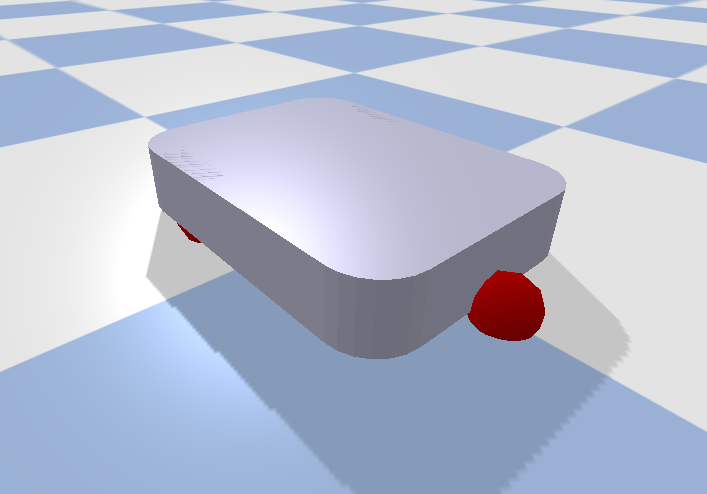
\includegraphics[width=5cm]{figures/boxer_robot.png}
    \caption{Pushing task through blocked corridor with the point robot, a green cube to push toward the target ghost state and a red blockade.}
    \label{fig:blocked_path_example_environment}
\end{figure}

\begin{figure}[H]
    \centering
    \begin{subfigure}{.5\textwidth}
    \centering
    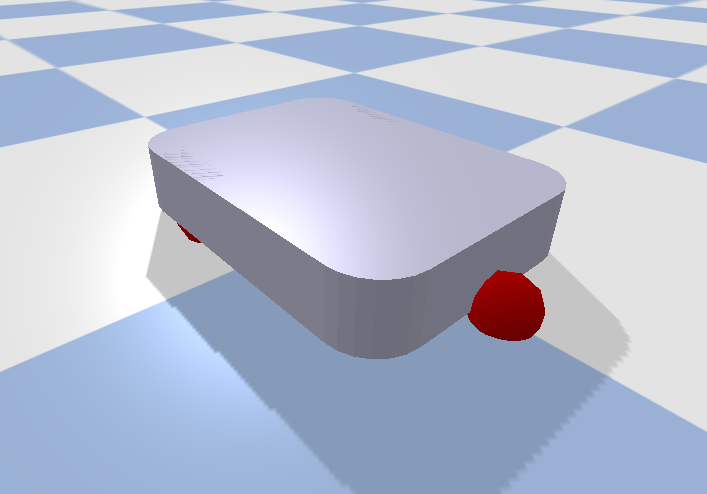
\includegraphics[width=0.8\textwidth]{figures/boxer_robot.png}
    \caption{todo}
    \label{subfig:todo}
    \end{subfigure}%

    \begin{subfigure}{.5\textwidth}
    \centering
    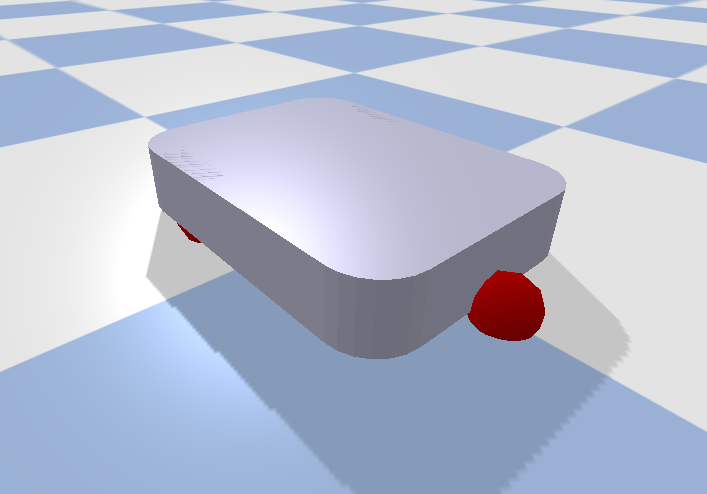
\includegraphics[width=0.8\textwidth]{figures/boxer_robot.png}
    \caption{todo}
    \label{subfig:B}
    \end{subfigure}
    \caption{todo}
    \label{subfig:blocked_path_hgraph_exmple}
\end{figure}

\todo[inline]{update the figure above here, Martijn did not like single/multi body, completely replace these terms.}
\todo[inline]{make the colors different, some which can be visualised with the airlab monitors.}

\todo[inline]{here are some example hgraph's required}

\todo[inline]{should I do an example Hgraph here? that requires target ghost positions. yes implement a }

As can be seen in \cref{tikz:flowchart_hgraph} there are some methods used which are still unexplained. Such as path non-existence, or motion planning. 
\todo[inline]{walk through the flowchart, what is actually happening here, It might be in your mind, but can the reader understand the flowchart without any additional context? clarify how edges are initialised, hypotheses are formed and how replanning occurs}


\subsection{Example}%
\label{subsec:hgraph_example}

\todo[inline]{here are some example hgraph's required}
\begin{figure}[H]
    \centering
    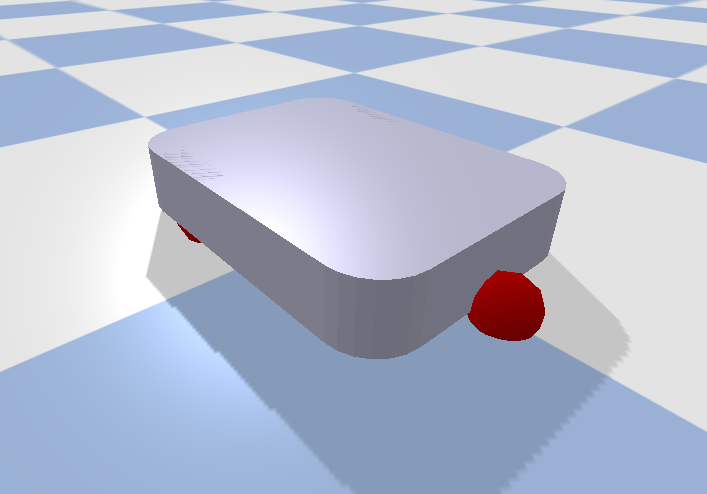
\includegraphics[width=5cm]{figures/boxer_robot.png}
    \caption{Pushing task through blocked corridor with the point robot, a green cube to push toward the target ghost state and a red blockade.}%
\label{fig:blocked_path_example_environment}
\end{figure}

\begin{figure}[H]
    \centering
    \begin{subfigure}{.5\textwidth}
    \centering
    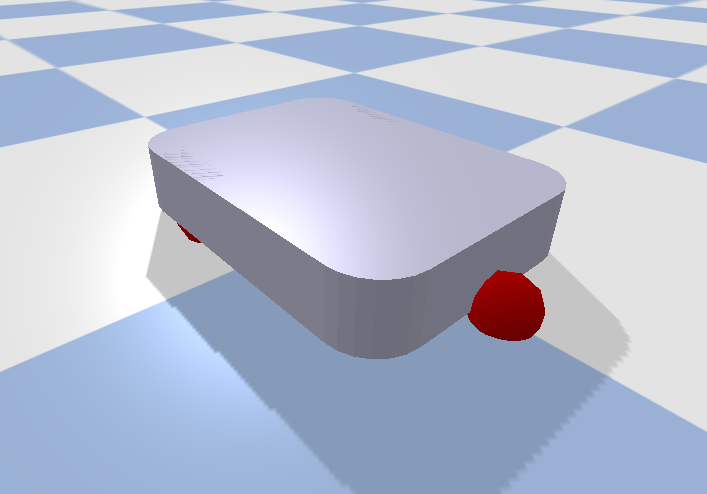
\includegraphics[width=0.8\textwidth]{figures/boxer_robot.png}
    \caption{todo}%
    \label{subfig:todo}
    \end{subfigure}%

    \begin{subfigure}{.5\textwidth}
    \centering
    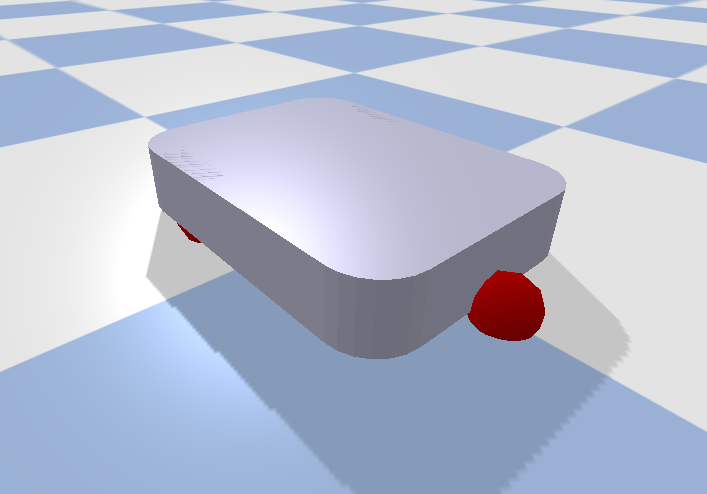
\includegraphics[width=0.8\textwidth]{figures/boxer_robot.png}
    \caption{todo}%
    \label{subfig:B}
    \end{subfigure}
    \caption{todo}%
    \label{subfig:blocked_path_hgraph_exmple}
\end{figure}



